\documentclass[12pt,a4paper]{article}
\usepackage[utf8]{inputenc}
\usepackage[spanish]{babel}
\usepackage{amsmath} 
\usepackage{amsfonts}
\usepackage{amssymb}
\usepackage{graphicx}
\usepackage{ragged2e}
\usepackage{multicol}
\usepackage{multirow}
\usepackage{booktabs}
\usepackage{float}
\usepackage{enumitem}
\usepackage[left=2.54cm,right=2.54cm,top=2.54cm,bottom=2.54cm]{geometry} 
\usepackage{titlesec}
\usepackage{hyperref}
\usepackage{xurl}
\usepackage{booktabs}
\usepackage{pgfplots}
\usepackage{floatrow}
\usepackage{listings}
\usepackage{inputenc}
\usepackage{fontenc}
\lstset{basicstyle=\ttfamily}
\titleformat*{\section}{\LARGE\bfseries}
\titleformat*{\subsection}{\Large\bfseries}
\titleformat*{\subsubsection}{\large\bfseries}
\titleformat*{\paragraph}{\large\bfseries}
\titleformat*{\subparagraph}{\large\bfseries}
\setcounter{topnumber}{20}
\setlength{\parindent}{0pt}
\renewcommand{\labelenumii}{\arabic{enumi}.\arabic{enumii}}
\renewcommand{\labelenumiii}{\arabic{enumi}.\arabic{enumii}.\arabic{enumiii}}
\renewcommand{\labelenumiv}{\arabic{enumi}.\arabic{enumii}.\arabic{enumiii}.\arabic{enumiv}}
% Configure bash
\lstdefinestyle{BashInputStyle}{
  language=bash,
  basicstyle=\small\sffamily,
  numbers=left,
  numberstyle=\tiny,
  numbersep=3pt,
  frame=tb,
  columns=fullflexible,
  linewidth=0.9\linewidth,
  xleftmargin=0.1\linewidth
}
\begin{document}

\thispagestyle{empty}

\newcommand{\HRule}{\rule{\linewidth}{0.5mm}}
 \center
 \textsc{\LARGE Universidad Nacional Autónoma de México} \\[0.5cm] \textsc{\Large Facultad de Ingeniería}\\
\begin{figure}[htb]
\centering

\includegraphics[width=8cm]{img/UNAM.jpg}
 \end{figure}
{\large PROTECO\\ \large{\bf GNU/Linux}\\ \vspace*{0.1cm} \vspace*{0.1cm} \vspace*{0.2cm} \vspace*{0.1cm} \HRule \\[0.4cm] { \LARGE \bfseries Terminal de trabajo PREBE} \\ \HRule \\[1cm]}
\large{\bf Equipo 9:}\\Rodríguez García Javier Antonio\\Treviño Selles Jorge Eithan\\
\vspace{0.5cm}\vspace{0.3cm} \large{\bf GENERACIÓN 44}\\
\vspace{0.5cm} {\Large \textsc{22 de abril del 2023}}\\
\newpage
\date{}
\justifying
\tableofcontents
\newpage

\section{Introducción}
\justifying
\noindent
Durante este proyecto se elaboró una terminal de trabajo utilizando el lenguaje de programación Bash; esta terminal de trabajo es capaz de ejecutar los comandos dentro de un sistema Linux además de que posee algunos comandos adicionales para ejecutar programas elaborados por nosotros como lo es un juego o un reproductor mp3. Todos estos programas nos han ayudado tanto a aplicar los conocimientos vistos en el curso así como a investigar y pensar en cómo resolver ciertas particularidades tanto de Bash como de Linux (sintaxis, dónde se encuentran ubicados ciertos archivos, manejo de procesos simultáneos, etc).
\\  

\noindent
El proyecto fue elaborado de forma colaborativa a lo largo de varios archivos con extensión .sh para así facilitar la modularidad y el trabajo en equipo. La colaboracion se realizó a través de GitHub: utilizamos una convención para nombrar los commits además de establecer normativas para trabajar con las diferentes versiones del proyecto, esto para asegurar que los avances realizados fueran coherentes y mantener una forma de trabajo organizada y fácil de mantener.
\section{Desarrollo}
\justifying
\noindent
En esta sección describiremos brevemente el funcionamiento de cada uno de los componentes que elaboramos para esta terminal de trabajo. Cada uno de estos comandos se encuenta almacenado en diferentes archivos .sh cuyo nombre sin la extensión es el mismo que el archivo que lo ejecuta.

\subsection{Sistema de acceso}
    \justifying
    \noindent
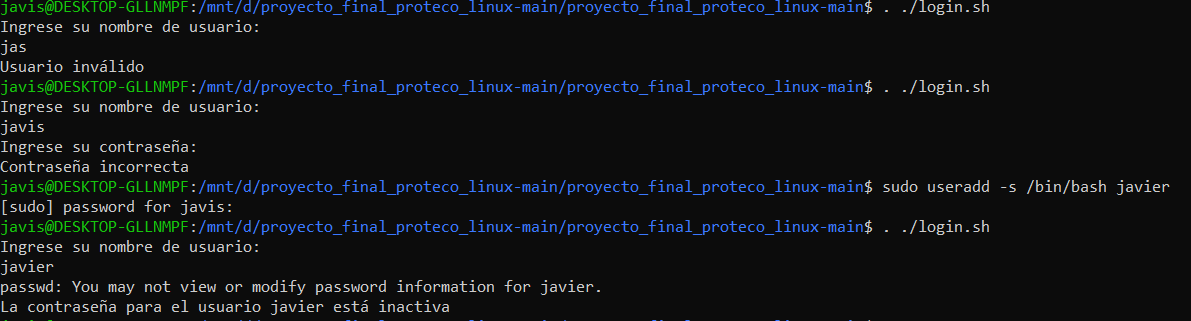
\includegraphics[width=14cm]{img/login1.png}\\
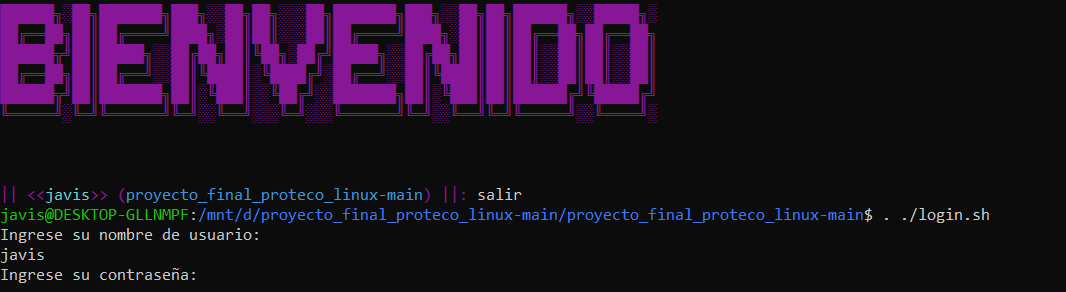
\includegraphics[width=14cm]{img/login2.png}
    Como se observa en la ejecucion se pueden precentar 4 casos al iniciar seción, en el priemrcaso, el usuario ingresado no existe en el sistema y por ende se devuelve un mensaje en el que se dice que usuario que no existe, en el segundo caso, el usuario existe, pero la contraseña ingresada no es correcta, el tercer caso se precenta cuando el usuario existe pero no cuenta con una contraseña, por ultimo, el cuarto caso se precenta cuando las credenciales son validas, una vez el usuario ingrese, aparecera el mensaje de bienvenida, (en la captura se coloco de esa manera devido a que el logearse implica un clear, lo que borra la informacion y no es posible visualizar como es que se realizo el logeo).\\\\
    \noindent
 \textbf{Explicación del código:}\\
    En el codigo se realizan 3 comparaciones, en la primera se comprueva que el usuario exista, esto lo hace mediante el comando "\textit{id}", etext  l cual arroja informacion del usuario, por lo que si el usuario no existe, al errojar un error, se activa el if, en ambos casos se cancela la salida que arroja el programa con el comando \text{ "&>/dev/null" }, la segunda comparacion se usa para saber si el usuario tiene contraseña, la tercera comparacion se hace intentando logearse nuevamente, de esta manera, si se permite logear no se entre en el if, pero si no se permite logear, entra en el if, y se dice que la contraseña es incorrecta
    \newpage
\textbf{Código:}
    \begin{lstlisting}[style=BashInputStyle]
 
#!/bin/bash

echo "Ingrese su nombre de usuario:"
read username

# Verificar si el usuario existe
if ! id "$username" &>/dev/null; then
  echo "Usuario inválido"
  return  
fi

if [[ $(passwd -S "$username" | awk '{print $2}') == "P" ]]; then
  echo "Ingrese su contraseña:"
  read -s password
  pass=1
  if ! echo "$password" | su - "$username" -c 'echo ""' >/dev/null 2>&1; then
    echo "Contraseña incorrecta"
    pass=0
  fi
else
  echo "La contraseña para el usuario $username está inactiva"
  pass=0
fi
if [ $pass -eq 1 ]
then
  tput setaf 1
  clear
  echo "
  
██████╗░
██╔══██╗
██████╦╝
██╔══██╗
██████╦╝
╚═════╝░"
sleep 0.2 
  tput setaf 2
  clear
  echo "
██████╗░██╗
██╔══██╗██║
██████╦╝██║
██╔══██╗██║
██████╦╝██║
╚═════╝░╚═╝"
  sleep 0.2
  tput setaf 3
  clear
  echo "
██████╗░██╗███████╗
██╔══██╗██║██╔════╝
██████╦╝██║█████╗░░
██╔══██╗██║██╔══╝░░
██████╦╝██║███████╗
╚═════╝░╚═╝╚══════╝"
  sleep 0.2
  tput setaf 4
  clear
  echo "
██████╗░██╗███████╗███╗░░██╗
██╔══██╗██║██╔════╝████╗░██║
██████╦╝██║█████╗░░██╔██╗██║
██╔══██╗██║██╔══╝░░██║╚████║
██████╦╝██║███████╗██║░╚███║
╚═════╝░╚═╝╚══════╝╚═╝░░╚══╝"
  sleep 0.2
  tput setaf 5
  clear
  echo "
██████╗░██╗███████╗███╗░░██╗██╗░░░██╗
██╔══██╗██║██╔════╝████╗░██║██║░░░██║
██████╦╝██║█████╗░░██╔██╗██║╚██╗░██╔╝
██╔══██╗██║██╔══╝░░██║╚████║░╚████╔╝░
██████╦╝██║███████╗██║░╚███║░░╚██╔╝░░
╚═════╝░╚═╝╚══════╝╚═╝░░╚══╝░░░╚═╝░░░"
  sleep 0.2 
  tput setaf 6
  clear
  echo "
██████╗░██╗███████╗███╗░░██╗██╗░░░██╗███████╗
██╔══██╗██║██╔════╝████╗░██║██║░░░██║██╔════╝
██████╦╝██║█████╗░░██╔██╗██║╚██╗░██╔╝█████╗░░
██╔══██╗██║██╔══╝░░██║╚████║░╚████╔╝░██╔══╝░░
██████╦╝██║███████╗██║░╚███║░░╚██╔╝░░███████╗
╚═════╝░╚═╝╚══════╝╚═╝░░╚══╝░░░╚═╝░░░╚══════╝"
  sleep 0.2
  tput setaf 7
  clear
  echo "
██████╗░██╗███████╗███╗░░██╗██╗░░░██╗███████╗███╗░░██╗
██╔══██╗██║██╔════╝████╗░██║██║░░░██║██╔════╝████╗░██║
██████╦╝██║█████╗░░██╔██╗██║╚██╗░██╔╝█████╗░░██╔██╗██║
██╔══██╗██║██╔══╝░░██║╚████║░╚████╔╝░██╔══╝░░██║╚████║
██████╦╝██║███████╗██║░╚███║░░╚██╔╝░░███████╗██║░╚███║
╚═════╝░╚═╝╚══════╝╚═╝░░╚══╝░░░╚═╝░░░╚══════╝╚═╝░░╚══╝"
  sleep 0.2 
  tput setaf 8
  clear
  echo "
██████╗░██╗███████╗███╗░░██╗██╗░░░██╗███████╗███╗░░██╗██╗
██╔══██╗██║██╔════╝████╗░██║██║░░░██║██╔════╝████╗░██║██║
██████╦╝██║█████╗░░██╔██╗██║╚██╗░██╔╝█████╗░░██╔██╗██║██║
██╔══██╗██║██╔══╝░░██║╚████║░╚████╔╝░██╔══╝░░██║╚████║██║
██████╦╝██║███████╗██║░╚███║░░╚██╔╝░░███████╗██║░╚███║██║
╚═════╝░╚═╝╚══════╝╚═╝░░╚══╝░░░╚═╝░░░╚══════╝╚═╝░░╚══╝╚═╝"
  sleep 0.2
  tput setaf 9
  clear
  echo "
██████╗░██╗███████╗███╗░░██╗██╗░░░██╗███████╗███╗░░██╗██╗██████╗░
██╔══██╗██║██╔════╝████╗░██║██║░░░██║██╔════╝████╗░██║██║██╔══██╗
██████╦╝██║█████╗░░██╔██╗██║╚██╗░██╔╝█████╗░░██╔██╗██║██║██║░░██║
██╔══██╗██║██╔══╝░░██║╚████║░╚████╔╝░██╔══╝░░██║╚████║██║██║░░██║
██████╦╝██║███████╗██║░╚███║░░╚██╔╝░░███████╗██║░╚███║██║██████╔╝
╚═════╝░╚═╝╚══════╝╚═╝░░╚══╝░░░╚═╝░░░╚══════╝╚═╝░░╚══╝╚═╝╚═════╝░"
  sleep 0.2 
clear
echo -e "\e[35m 
██████╗░██╗███████╗███╗░░██╗██╗░░░██╗███████╗███╗░░██╗██╗██████╗░░█████╗░
██╔══██╗██║██╔════╝████╗░██║██║░░░██║██╔════╝████╗░██║██║██╔══██╗██╔══██╗
██████╦╝██║█████╗░░██╔██╗██║╚██╗░██╔╝█████╗░░██╔██╗██║██║██║░░██║██║░░██║
██╔══██╗██║██╔══╝░░██║╚████║░╚████╔╝░██╔══╝░░██║╚████║██║██║░░██║██║░░██║
██████╦╝██║███████╗██║░╚███║░░╚██╔╝░░███████╗██║░╚███║██║██████╔╝╚█████╔╝
╚═════╝░╚═╝╚══════╝╚═╝░░╚══╝░░░╚═╝░░░╚══════╝╚═╝░░╚══╝╚═╝╚═════╝░░╚════╝░\e[0m"

echo ''
    echo ""
    echo ""
. ./linea-comando.sh
fi
    \end{lstlisting} 
\newpage   
\justifying
\subsection{Línea de comandos}
    \centering
    
\includegraphics[width=14cm]{img/linea-comando.png} \\
    \justifying
    \noindent
    Tras iniciar sesión, tendremos acceso a la línea de comando; dentro de ella podemos ingresar cualquier comando de Linux y se ejecutará como si se trata de la terminal Bash estandár además de poder también tener acceso a todos los comandos que hemos creado en este proyecto.
    \\\\
    Dentro de la línea de comandos podremos ver el usuario que está utilizando el sistema actualmente así como el directorio donde se encuentra actualmente.
    \\\\
    Un aspecto importante a considerar es que la principal forma para salir de esta terminal es utilizando la siguiente sentencia:
    \\
    \textbf{Código:}
    \begin{lstlisting}[style=BashInputStyle]
#!/bin/bash
# Overwrite the exit command
exit() {
    :
}
# Overwrite the default trap for SIGTSTP, SIGINT and SIGTERM
trap ' ' SIGTSTP SIGINT SIGTERM
while true
do
    # Get current directory, and replace home directory with ~
    DIR=$( basename "$PWD" | sed "s|$HOME|~|" )
    
    # Show prompt with colors and read input
    printf "\e[35m|| <<\e[1;36m$USER\e[0m\e[35m>> (\e[36m$DIR\e[35m) ||: \e[0m"
    read input
    
    # If command with the specified name exists inside the current directory, execute the script
    if [ -e "$(echo $input | cut -d ' ' -f1).sh" ]
    then
        if echo $input | grep -q " "; then
            source "./$(echo $input | cut -d ' ' -f1).sh" "$(echo $input | cut -d ' ' -f2)"
        else
	        source "./$input.sh"
        fi    
    # If input is "salir", exit the loopd
    elif [ "$input" == "salir" ]
    then
	break

    # Execute OS command
    else
	$input
    fi
done

# Return to the default trap for SIGTSTP, SIGINT and SIGTERM
trap - SIGTSTP SIGINT SIGTERM
    \end{lstlisting} 
    \justifying
    \noindent
    \\Los comandos \textit{exit}, \textit{CTRL+C}, \textit{CTRL+X} y \textit{CTRL+Z} están desactivados dentro de esta terminal.
    \\\\
    \noindent
    \textbf{Explicación del código:}\\
    Primero sobreescribe las sentencias \textit{exit}, \textit{CTRL+C}, \textit{CTRL+X} y \textit{CTRL+Z} para prevenir que puedan ejecutarse. Posteriormente se entra en un ciclo eterno que muestra primero el usuario y directorio actual para después leer un string del usuario: primero se determinará si los caracteres antes del espacio de este string corresponden a uno de los comandos; en caso de que lo sea se determinará si este tiene un atributo para correr ya sea el script normal (agregando .sh a dicho comando y ejecutandólo) o dividir el string para una parte utilizarla para la ejecución y la otra para argumento. Si no se trata de un comando que hayamos realizado, se ejecutará directamente como si fuera una terminal de bash estandár. Al finalizar, se liberan las sentencias \textit{exit}, \textit{CTRL+C}, \textit{CTRL+X} y \textit{CTRL+Z} que habían sido reservadas
\newpage
\justifying
\subsection{Ayuda}
    \centering
    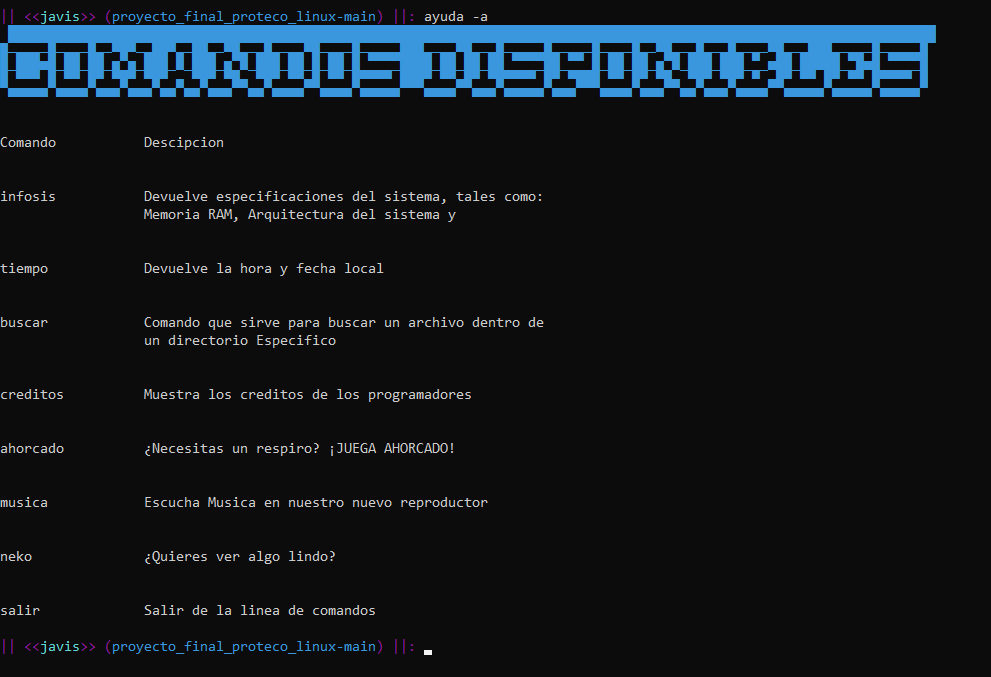
\includegraphics[width=8cm]{img/ayuda1.png} \\
    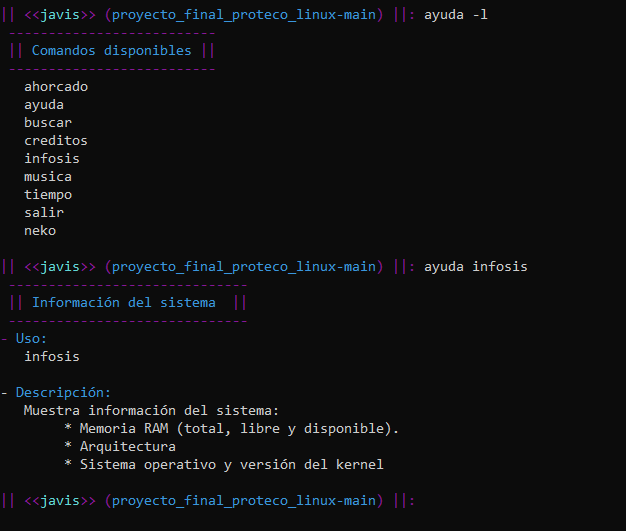
\includegraphics[width=8cm]{img/ayuda2.png}

    \justifying
    \noindent
    \\
    Este comando proporciona informacion de los comandos que se programaron para el proyecto, en este se tienen diferentes opciones, para poder utilizarlo se debe escribir \textit{ayuda} seguido del comando del que se necesita la ayuda, ademas de que se pueden agregar las banderas \textit{-a} para 
    visualizar una descripcion general de todos los comandos y \textit{-l} para visualizar unicamente los comandos que se pueden utilizar, sin ninguna descripción.
    \\
    \textbf{Código:}
    \begin{lstlisting}[style=BashInputStyle]
#!/bin/bash
# Check if user has given an argument, if not, ask it
if [ -z $1 ] ; then
    echo ""
    read -p $'\e[35m-> \e[36mIngrese el comando del cual necesitas ayuda: \e[0m'  command
else 
    command=$1
fi
if [ -z $command ] ; then
    echo -e "\e[31m-> ERROR: No se ingresó ningún comando"
else 
    # Check if command was created by us
    case $command in
        "-a" ) # Descripción de todos los comandos
            echo -e "\e[36m ascii art\e[0m"

printf "\n\n"
echo "Comando           Descipcion"
printf "\n\n"
echo "infosis           Devuelve especificaciones del sistema, tales como:"
echo "                  Memoria RAM, Arquitectura del sistema y "
printf "\n\n"
echo "tiempo            Devuelve la hora y fecha local"
printf "\n\n"
echo "buscar            Comando que sirve para buscar un archivo dentro de"
echo "                  un directorio Especifico"
printf "\n\n"
echo "creditos          Muestra los creditos de los programadores"
printf "\n\n"
echo "ahorcado          ¿Necesitas un respiro? ¡JUEGA AHORCADO!"
printf "\n\n"
echo "musica            Escucha Musica en nuestro nuevo reproductor"
printf "\n\n"
echo "neko              ¿Quieres ver algo lindo?"
printf "\n\n"
echo "salir             Salir de la linea de comandos"
        ;;
    "-l" ) # Lista de comandos disponibles
        echo -e "\e[35m --------------------------"
        echo -e " || \e[36mComandos disponibles \e[35m||"
        echo -e " --------------------------\e[0m"
        echo -e "   ahorcado"    
        echo -e "   ayuda"
        echo -e "   buscar"
        echo -e "   creditos"
        echo -e "   infosis"
        echo -e "   musica"
        echo -e "   tiempo"
        echo -e "   salir"
        echo -e "   neko"
        ;;
    "ahorcado" ) # Juego ahorcado
        echo -e "\e[35m ---------------"
        echo -e " || \e[36mAhorcado  \e[35m||"
        echo -e " ---------------"
        echo -e "- \e[36mUso: \e[0m"
        echo -e "   ahorcado \e[0m"
        echo ""
        echo -e "- \e[36mDescripción: \e[0m"
        echo -e "   Se ejecuta el juego del ahorcado: se trata de adivinar una 
        palabra secreta, ingresando letras. Si se adivina la palabra, se gana.
        Si se adivina la palabra, se pierde."
        ;;
    "ayuda" ) # Comando de ayuda
        echo -e "\e[35m -----------------------"
        echo -e " || \e[36mComando de ayuda  \e[35m||"
        echo -e " -----------------------"
        echo -e "- \e[36mUso: \e[0m"
        echo -e "   ayuda \e[0m"
        echo -e "   ayuda \e[1mcomando_a_consultar\e[0m"
        echo -e "   ayuda \e[1m-l\e[0m (ver lista de comandos disponibles))"
        echo -e "   ayuda \e[1m-a\e[0m (ver descripción todos los comandos
        disponibles)"
        echo ""
        echo -e "- \e[36mDescripción: \e[0m"
        echo -e "   Muestra la información de un comando creado por nosotros."  
        ;;
    "buscar" ) # Comando de búsqueda
        echo -e "\e[35m --------------------------"
        echo -e " || \e[36mComando de búsqueda  \e[35m||"
        echo -e " --------------------------"
        echo -e "- \e[36mUso: \e[0m"
        echo -e "   buscar"
        echo -e "   buscar \e[1;36mdirectorio_donde_buscar\e[0m"
        echo -e "   buscar \e[1;36mdirectorio_donde_buscar archivo_a_buscar\e[0m"
        echo ""
        echo -e "- \e[36mDescripción: \e[0m"
        echo -e "   Busca un archivo en el sistema de archivos: si lo encuentra
        muestra un mensaje de éxito, si no lo encuentra muestra que no lo 
        encontró y si el directorio no existe muestra un mensaje de error."
        ;;
    "creditos" ) # Comando para ver créditos de los autores
        echo -e "\e[35m ------------------------------"
        echo -e " || \e[36mCréditos de los autores  \e[35m||"
        echo -e " ------------------------------"
        echo -e "- \e[36mUso: \e[0m"
        echo -e "   creditos \e[0m"
        echo ""
        echo -e "- \e[36mDescripción: \e[0m"
        echo -e "   Muestra los créditos de los autores del proyecto y un
        personaje de Among Us."
        ;;
    "infosis" ) # Comando para ver información del sistema
        echo -e "\e[35m ------------------------------"
        echo -e " || \e[36mInformación del sistema  \e[35m||"
        echo -e " ------------------------------"
        echo -e "- \e[36mUso: \e[0m"
        echo -e "   infosis \e[0m"
        echo ""
        echo -e "- \e[36mDescripción: \e[0m"
        echo -e "   Muestra información del sistema:
        * Memoria RAM (total, libre y disponible).
        * Arquitectura
        * Sistema operativo y versión del kernel"
            ;;
    "musica" ) # Reproductor de mp3
        echo -e "\e[35m -------------------------"
        echo -e " || \e[36mReproductor de mp3  \e[35m||"
        echo -e " -------------------------"
        echo -e "- \e[36mUso: \e[0m"
        echo -e "   musica \e[0m"
        echo -e "   musica \e[1mdirectorio_con_mp3\e[0m"
        echo ""
        echo -e "- \e[36mDescripción: \e[0m"
        echo -e "   Abre un reproductor de música en el directorio 
        especificado que permite reproducir archivos mp3. Si no se
        especifica un directorio, se abre en el directorio actual."
            ;;
        
    "tiempo" )  # Ver tiempo actual
        echo -e "\e[35m ---------------------------------"
        echo -e " || \e[36mComando para ver el tiempo  \e[35m||"
        echo -e " ---------------------------------"
        echo -e "- \e[36mUso: \e[0m"
        echo -e "   tiempo \e[0m"
        echo ""
        echo -e "- \e[36mDescripción: \e[0m"
        echo -e "   Muestra la hora y fecha actual."
            ;;
    "salir") #salir de la linea de 
        echo -e "\e[35m ---------------------------------"
        echo -e " || \e[36m Comando para finalizar la ejecucion \e[35m||"
        echo -e " ---------------------------------"
        echo -e "- \e[36mUso: \e[0m"
        echo -e "   finalizar ejecucion del programa \e[0m"
        echo ""
        echo -e "- \e[36mDescripción: \e[0m"
        echo -e "   Es el comando unico para poder finalizar la ejecucion del
        programa y salir a la terminal nativa del sistema."
            ;;
    "neko") #imprimer un neko
        echo -e "\e[35m ---------------------------------"
        echo -e " || \e[36m Comando para ver un lindo neko\e[35m||"
        echo -e " ---------------------------------"
        echo -e "- \e[36mUso: \e[0m"
        echo -e "   ver un lindo gato, (se recomienda reducir el tamano de las
        letras) \e[0m"
        echo ""
        echo -e "- \e[36mDescripción: \e[0m"
        echo -e "   ¿La tarea o el trabajo te tienen estresado?  ¡Ve un lindo
        gato y olvida tus problemas!"
        ;;
    * ) # Cualquier otro input
        echo ""
        echo -e "\e[35m-> \e[31mLa información de este comando no está 
        disponible con "ayuda""
        echo -e "\e[35m-> \e[36mPara ver la lista de comandos disponible,
        ejecute \e[1;36mayuda -l\e[0m"
        ;;
    esac
    echo ""
fi
    \end{lstlisting} 
    \textbf{Sintaxis:}
    \begin{lstlisting}[style=BashInputStyle]
ayuda
ayuda comando_a_consultar
    \end{lstlisting} 
    \justifying
    \noindent
Para el funcionamiento del codigo se implementaron 2 if: el primero comprueba si ya se coloco un argumento al comando; si este argumento esta vacio  (es decir, en la terminale se colocó únicamente ayuda), le pide al usuario que introduzca el comando del que se quiere obtener la ayuda; el segundo if esta colocado para comprobar que se haya colocado algún comando, en caso de que no se haya colocado se devolverá un mensaje de error; si se coloco algun comando se ingresará a una estructura \textit{case} en la que dependiendo del comando que se escribió se devolverá la información correspondiente, en caso de colocar un comando que no exista se devolverá un mensaje informando al usuario.
\justifying
\newpage
\subsection{Información del sistema}
    \centering
    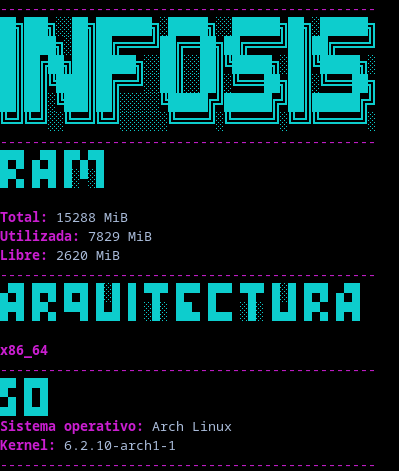
\includegraphics[width=8cm]{img/infosis.png}
    \\
    \justifying
    \noindent
    Al ejecutar este comando \textit{infosis} se muestra en pantalla información acerca del sistema que estamos utilizando:
    \begin{itemize}
        \item \textbf{RAM} \\
        Se muestra la memoria RAM total, utilizada y libre del sistema utilizando megabytes (MiB) como unidades.
        \item \textbf{Arquitectura} \\
        Se muestra la arquitectura que utiliza nuestro sistema.
        \item \textbf{SO} \\
        Se muestra el nombre de nuestro sistema operativo así como la versión del kernel que estamos utilizando.
    \end{itemize}
    
    \textbf{Código:}
    \\
    \begin{lstlisting}[style=BashInputStyle]
## Cool logo
echo -e "\e[35m
-----------------------------------------------
\e[36m██╗███╗░░██╗███████╗░█████╗░░██████╗██╗░██████╗
██║████╗░██║██╔════╝██╔══██╗██╔════╝██║██╔════╝
██║██╔██╗██║█████╗░░██║░░██║╚█████╗░██║╚█████╗░
██║██║╚████║██╔══╝░░██║░░██║░╚═══██╗██║░╚═══██╗
██║██║░╚███║██║░░░░░╚█████╔╝██████╔╝██║██████╔╝
╚═╝╚═╝░░╚══╝╚═╝░░░░░░╚════╝░╚═════╝░╚═╝╚═════╝░
\e[35m-----------------------------------------------"


## RAM Usage
echo -e "\e[36m█▀█ ▄▀█ █▀▄▀█
█▀▄ █▀█ █░▀░█
"
# Get the memory usage in MiB and filter the output to only show the Mem row
mem_info=$(free -m | grep Mem)

# Extract the total used and free memory values as strings
total_mem=$(echo $mem_info | awk '{print $2}')
used_mem=$(echo $mem_info | awk '{print $3}')
free_mem=$(echo $mem_info | awk '{print $4}')

# Show memory values
echo -e "\e[1;35mTotal:\e[0m $total_mem MiB"
echo -e "\e[1;35mUtilizada:\e[0m $used_mem MiB"
echo -e "\e[1;35mLibre:\e[0m $free_mem MiB"


## System Architecture
echo -e "\e[35m-----------------------------------------------\e[36m
▄▀█ █▀█ █▀█ █░█ █ ▀█▀ █▀▀ █▀▀ ▀█▀ █░█ █▀█ ▄▀█
█▀█ █▀▄ ▀▀█ █▄█ █ ░█░ ██▄ █▄▄ ░█░ █▄█ █▀▄ █▀█"
architecture=$(uname -m)
echo -e "
\e[1;35m$architecture\e[0m"

## OS Version
echo -e "\e[35m-----------------------------------------------\e[36m
█▀ █▀█
▄█ █▄█"

# Extract OS name and Kernel
os_name=$(sed -n 's/PRETTY_NAME="\(.*\)"/\1/p' /etc/os-release)
kernel=$(uname -r)

# Show values
echo -e "\e[1;35mSistema operativo:\e[0m $os_name"
echo -e "\e[1;35mKernel:\e[0m $kernel"
echo -e "\e[35m-----------------------------------------------\e[0m
"
    \end{lstlisting}
    
    \\
    \noindent
    \textbf{Sintaxis:} \\
    \begin{lstlisting}[style=BashInputStyle]
infossis
    \end{lstlisting}
    \noindent
    \textbf{Explicación del código:} \\
    \noindent
    Para obtener la memoria RAM se utiliza el comando free y después se muestra sólo la información necesaria (esta es extraída utilizando la herramienta awk. La arquitectura se consigue utilizando el comando \textit{\$(uname -m)}. Finalmente, para obtener el nombre y kernel del sistema operativo utilizamos primero el programa \textit{sed} para obtener el nombre de la distribución y después \textit{\$(uname -r} para obtener el kernel. Toda esta informacioń se muestra en pantalla.
    
\justifying
\subsection{Fecha y hora}
    \centering
    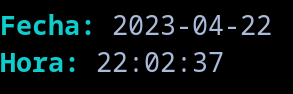
\includegraphics[width=8cm]{img/tiempo.png}
    \\
    \justifying
    \noindent
    Al ingresar el comando \textit{tiempo} se mostrará en pantalla la fecha y hora del sistema al instante.
    \\\\
    \textbf{Código:}
    \\
    \begin{lstlisting}[style=BashInputStyle]
printf "\n\e[1;36mFecha:\e[0m "
cat /sys/class/rtc/rtc0/date
printf "\e[1;36mHora:\e[0m "
cat /sys/class/rtc/rtc0/time
echo ""
    \end{lstlisting}
    \textbf{Sintaxis:}
    \\
    \begin{lstlisting}[style=BashInputStyle]
tiempo
    \end{lstlisting}
    \noindent
    \textbf{Explicación del código:} \\
    Imprime en pantalla el contenido de los archivos \textit{/sys/class/rtc/rtc0/time} y \textit{/sys/class/rtc/rtc0/date}.
\newpage
\justifying
\subsection{Buscar}
    \justifying
    \noindent
    El comando buscar nos permite saber si un archivo se encuentra o no en un directorio especificado. Existen diferentes variantes de este programa ya que puede o no tomar argumentos: podemos especificar directamente en terminal el directorio y archivo a buscar o podemos también darlo de forma manual tras ejecutar el comando.
    \\
    
    \centering
    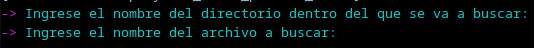
\includegraphics[width=10cm]{img/buscar_input.png}
    \\
    
\includegraphics[width=10cm]{img/buscar_found.png}
    \\\\

    \justifying
    \noindent
    Si el directorio no existe se le indicará al usuario en pantalla.
    \\

    \centering
    
\includegraphics[width=10cm]{img/buscar_no_dir.png}
    \\
    
    \justifying
    \noindent
    El programa buscará dentro del directorio si se encuentra o no el archivo en dicho directorio le dirá al usuario si lo encontró o no.
    \\\\

    \centering
    
\includegraphics[width=10cm]{img/buscar_not_found.png}
    \\\\

    \noindent
    \justifying
    \textbf{Código:}
    \\
    \begin{lstlisting}[style=BashInputStyle]
#!/bin/bash
function search()
{
	if [ -d $1 ] ; then
		if [[ -f "$1/$2" ]]; then
			echo -e "\n\e[92m	EL ARCHIVO SI ESTA EN EL DIRECTORIO"
		else 
			echo -e "\n\e[33m	EL ARCHIVO NO ESTA EN EL ESE DIRECTORIO"
		fi
	else
		echo -e "\n\e[31m	!!! NO EXISTE ESE DIRECTORIO !!!"
	fi
}
if [ $1 ]; then
	if [ $2 ] ; then
		search $1 $2
	else
		read -p $'\e[35m-> \e[36mIngrese el nombre del archivo que se va a buscar: \e[0m'  dir
		search $1 $dir
	fi
else 
	read -p $'\e[35m-> \e[36mIngrese el nombre del directorio dentro del que se va a buscar: \e[0m'  dir
	read -p $'\e[35m-> \e[36mIngrese el nombre del archivo a buscar: \e[0m'  file
	search $dir $file
fi
echo -e "\e[0m"
    \end{lstlisting}

    \textbf{Sintaxis:}
    \begin{lstlisting}[style=BashInputStyle]
buscar
buscar directorio
buscar directorio archivo
    \end{lstlisting}
    \textbf{Explicación del código:} \\
    Primero lee la entrada del usuario (ya sea que se le haya dado por terminal o pidiendóla directamente) y después averigua si se encuentra del archivo utilizando la bandera \textit{-f} para después mostrar el mensaje en pantalla si es que lo encontró.

\justifying
\subsection{Créditos}
    \centering
    
\includegraphics[width=6cm]{img/creditos.png}
    \\
    \justifying
    \noindent
    Cuando ejecutamos el comando \textit{creditos} se mostrará un mensaje con los nombres de los autores de esta terminal seguido de una figura de Among Us.
    \\\\
    \newpage
    \textbf{Código:}
    \\
    \begin{lstlisting}[style=BashInputStyle]
#!/bin/bash
echo -e "\e[35m
------------------------------------------------------------\e[36m
░█████╗░██████╗░███████╗██████╗░██╗████████╗░█████╗░░██████╗
██╔══██╗██╔══██╗██╔════╝██╔══██╗██║╚══██╔══╝██╔══██╗██╔════╝
██║░░╚═╝██████╔╝█████╗░░██║░░██║██║░░░██║░░░██║░░██║╚█████╗░
██║░░██╗██╔══██╗██╔══╝░░██║░░██║██║░░░██║░░░██║░░██║░╚═══██╗
╚█████╔╝██║░░██║███████╗██████╔╝██║░░░██║░░░╚█████╔╝██████╔╝
░╚════╝░╚═╝░░╚═╝╚══════╝╚═════╝░╚═╝░░░╚═╝░░░░╚════╝░╚═════╝░\e[35m
------------------------------------------------------------\e[36m
░░█ ▄▀█ █░█ █ █▀▀ █▀█   ▄▀█ █▄░█ ▀█▀ █▀█ █▄░█ █ █▀█
█▄█ █▀█ ▀▄▀ █ ██▄ █▀▄   █▀█ █░▀█ ░█░ █▄█ █░▀█ █ █▄█
█▀█ █▀█ █▀▄ █▀█ █ █▀▀ █░█ █▀▀ ▀█   █▀▀ ▄▀█ █▀█ █▀▀ █ ▄▀█
█▀▄ █▄█ █▄▀ █▀▄ █ █▄█ █▄█ ██▄ █▄   █▄█ █▀█ █▀▄ █▄▄ █ █▀█
░░█ █▀█ █▀█ █▀▀ █▀▀   █▀▀ █ ▀█▀ █░█ ▄▀█ █▄░█
█▄█ █▄█ █▀▄ █▄█ ██▄   ██▄ █ ░█░ █▀█ █▀█ █░▀█
▀█▀ █▀█ █▀▀ █░█ █ █▄░█ █▀█   █▀ █▀▀ █░░ █░░ █▀▀ █▀
░█░ █▀▄ ██▄ ▀▄▀ █ █░▀█ █▄█   ▄█ ██▄ █▄▄ █▄▄ ██▄ ▄█
\e[31m
	⠀⠀⠀⠀⠀⠀⠀⠀⠀⠀⠀⣠⣤⣤⣤⣤⣤⣶⣦⣤⣄⡀⠀⠀⠀⠀⠀⠀⠀⠀ 
	⠀⠀⠀⠀⠀⠀⠀⠀⢀⣴⣿⡿⠛⠉⠙⠛⠛⠛⠛⠻⢿⣿⣷⣤⡀⠀⠀⠀⠀⠀ 
	⠀⠀⠀⠀⠀⠀⠀⠀⣼⣿⠋⠀⠀⠀⠀⠀⠀⠀⢀⣀⣀⠈⢻⣿⣿⡄⠀⠀⠀⠀ 
	⠀⠀⠀⠀⠀⠀⠀⣸⣿⡏⠀⠀⠀⣠⣶⣾⣿⣿⣿⠿⠿⠿⢿⣿⣿⣿⣄⠀⠀⠀ 
	⠀⠀⠀⠀⠀⠀⠀⣿⣿⠁⠀⠀⢰⣿⣿⣯⠁⠀⠀⠀⠀⠀⠀⠀⠈⠙⢿⣷⡄⠀ 
	⠀⠀⣀⣤⣴⣶⣶⣿⡟⠀⠀⠀⢸⣿⣿⣿⣆⠀⠀⠀⠀⠀⠀⠀⠀⠀⠀⣿⣷⠀ 
	⠀⢰⣿⡟⠋⠉⣹⣿⡇⠀⠀⠀⠘⣿⣿⣿⣿⣷⣦⣤⣤⣤⣶⣶⣶⣶⣿⣿⣿⠀ 
	⠀⢸⣿⡇⠀⠀⣿⣿⡇⠀⠀⠀⠀⠹⣿⣿⣿⣿⣿⣿⣿⣿⣿⣿⣿⣿⣿⡿⠃⠀ 
	⠀⣸⣿⡇⠀⠀⣿⣿⡇⠀⠀⠀⠀⠀⠉⠻⠿⣿⣿⣿⣿⡿⠿⠿⠛⢻⣿⡇⠀⠀ 
	⠀⣿⣿⠁⠀⠀⣿⣿⡇⠀⠀⠀⠀⠀⠀⠀⠀⠀⠀⠀⠀⠀⠀⠀⠀⢸⣿⣧⠀⠀ 
	⠀⣿⣿⠀⠀⠀⣿⣿⡇⠀⠀⠀⠀⠀⠀⠀⠀⠀⠀⠀⠀⠀⠀⠀⠀⢸⣿⣿⠀⠀ 
	⠀⣿⣿⠀⠀⠀⣿⣿⡇⠀⠀⠀⠀⠀⠀⠀⠀⠀⠀⠀⠀⠀⠀⠀⠀⢸⣿⣿⠀⠀ 
	⠀⢿⣿⡆⠀⠀⣿⣿⡇⠀⠀⠀⠀⠀⠀⠀⠀⠀⠀⠀⠀⠀⠀⠀⠀⢸⣿⡇⠀⠀ 
	⠀⠸⣿⣧⡀⠀⣿⣿⡇⠀⠀⠀⠀⠀⠀⠀⠀⠀⠀⠀⠀⠀⠀⠀⠀⣿⣿⠃⠀⠀ 
	⠀⠀⠛⢿⣿⣿⣿⣿⣇⠀⠀⠀⠀⠀⣰⣿⣿⣷⣶⣶⣶⣶⠶⠀⢠⣿⣿⠀⠀⠀ 
	⠀⠀⠀⠀⠀⠀⠀⣿⣿⠀⠀⠀⠀⠀⣿⣿⡇⠀⣽⣿⡏⠁⠀⠀⢸⣿⡇⠀⠀⠀ 
	⠀⠀⠀⠀⠀⠀⠀⣿⣿⠀⠀⠀⠀⠀⣿⣿⡇⠀⢹⣿⡆⠀⠀⠀⣸⣿⠇⠀⠀⠀ 
	⠀⠀⠀⠀⠀⠀⠀⢿⣿⣦⣄⣀⣠⣴⣿⣿⠁⠀⠈⠻⣿⣿⣿⣿⡿⠏⠀⠀⠀⠀ 
	⠀⠀⠀⠀⠀⠀⠀⠈⠛⠻⠿⠿⠿⠿⠋⠁⠀⠀⠀⠀⠀⠀⠀⠀⠀⠀\e[35m⠀
------------------------------------------------------------\e[0m
"
    \end{lstlisting}
    \newpage
    \noindent
    \justifying
    \textbf{Sintaxis:}
    \begin{lstlisting}[style=BashInputStyle]
creditos
    \end{lstlisting}
    \textbf{Explicación del código:} \\
    Muestra los nombres de los creadores y un Among Us en pantalla con ASCII art.

 
\justifying
\subsection{Juego (ahorcado)}
  \centering
    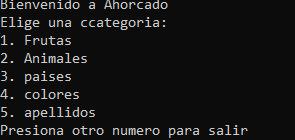
\includegraphics[width=8cm]{img/ahorcado1.png}\\
     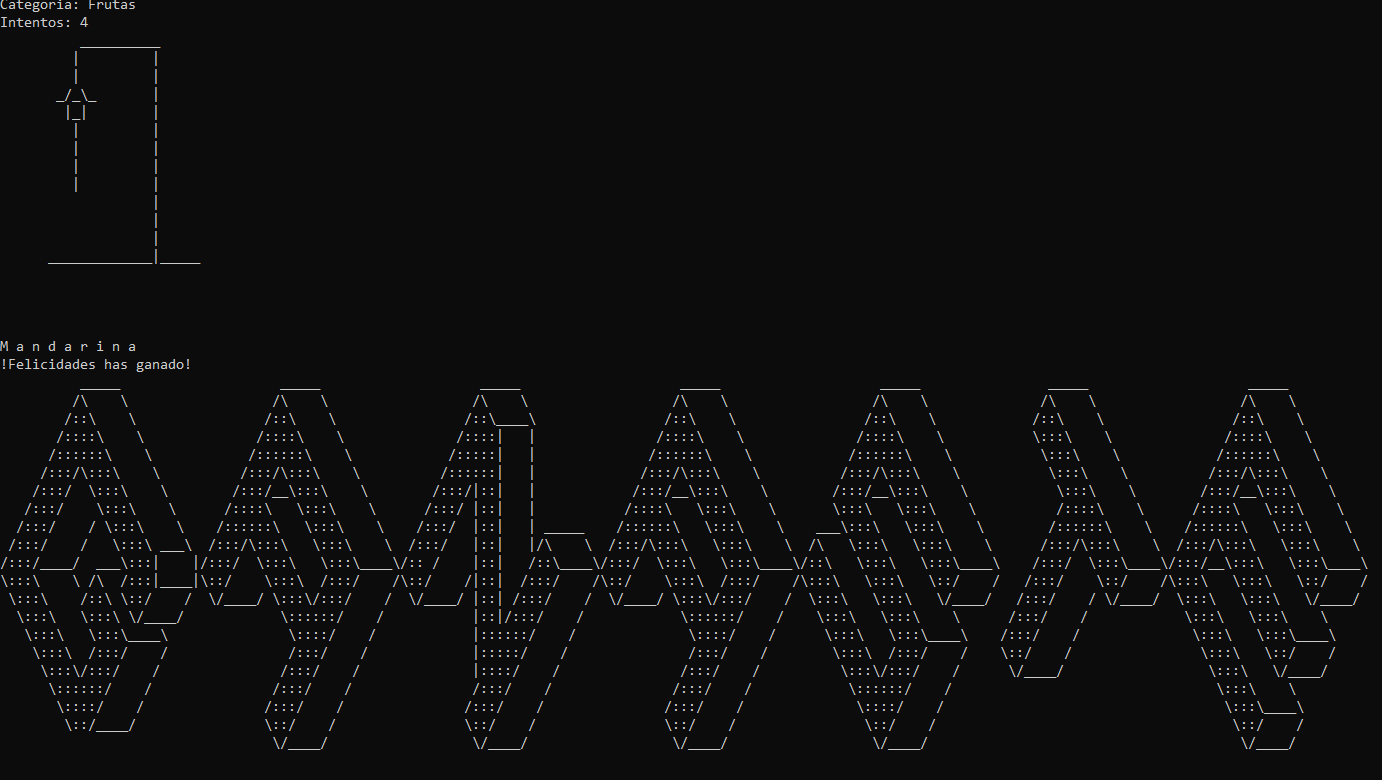
\includegraphics[width=8cm]{img/ahorcado2.png}\\
      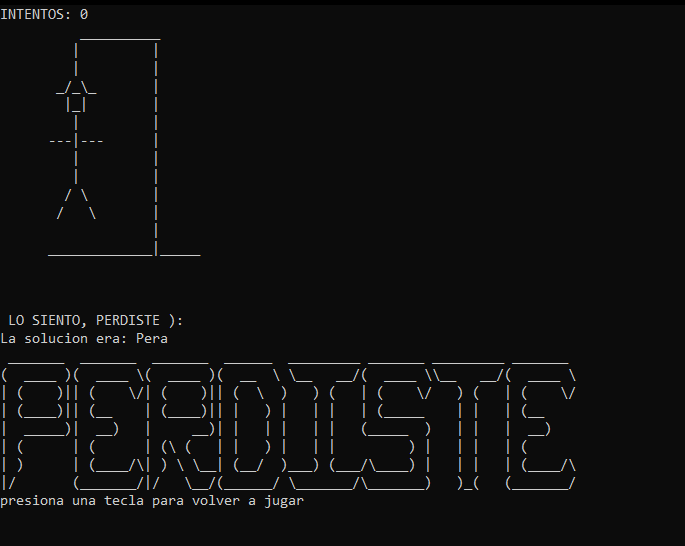
\includegraphics[width=8cm]{img/ahorcado3.png}\\
    \justifying
    \noindent
    lL primero que aparece cuando se ejecuta el juego es un menu, en el que el usuario puede elegir la tema del que se adivinara la palabra, una vez elegido el tema se precentan 6 vidas y la interfaz del juego, dependiendo de si ganes o pierdas se precentaran dos interfaces, una felicitandote y otra en donde se le informara al usuario que se quedo sin vidas
    \textbf{Código:}
     \begin{lstlisting}[style=BashInputStyle]
    #!/bin/bash
function dibujo {
    case $1 in
    0)
    echo "          __________"
echo "         |         |"
echo "         |         |"
echo "       _/_\_       |"
echo "        |_|        |"
echo "         |         |"
echo "      ---|---      |"
echo "         |         |"
echo "         |         |"
echo "        / \        |"
echo "       /   \       |"
echo "                   |"
echo "      _____________|_____"
echo "                           "
        ;;
    1)
        echo "          __________"
echo "         |         |"
echo "         |         |"
echo "       _/_\_       |"
echo "        |_|        |"
echo "         |         |"
echo "      ---|---      |"
echo "         |         |"
echo "         |         |"
echo "        /          |"
echo "       /           |"
echo "                   |"
echo "      _____________|_____"
echo "                           "
        ;;
    2)
       echo "          __________"
echo "         |         |"
echo "         |         |"
echo "       _/_\_       |"
echo "        |_|        |"
echo "         |         |"
echo "      ---|---      |"
echo "         |         |"
echo "         |         |"
echo "                   |"
echo "                   |"
echo "                   |"
echo "      _____________|_____"
echo "                           "
        ;;
    3)
echo "          __________"
echo "         |         |"
echo "         |         |"
echo "       _/_\_       |"
echo "        |_|        |"
echo "         |         |"
echo "      ---|         |"
echo "         |         |"
echo "         |         |"
echo "                   |"
echo "                   |"
echo "                   |"
echo "      _____________|_____"
echo "                           "
        ;;
    4)
       echo "          __________"
echo "         |         |"
echo "         |         |"
echo "       _/_\_       |"
echo "        |_|        |"
echo "         |         |"
echo "         |         |"
echo "         |         |"
echo "         |         |"
echo "                   |"
echo "                   |"
echo "                   |"
echo "      _____________|_____"
echo "                           "
        ;;
    5)
        echo "          __________"
echo "         |         |"
echo "         |         |"
echo "       _/_\_       |"
echo "        |_|        |"
echo "                   |"
echo "                   |"
echo "                   |"
echo "                   |"
echo "                   |"
echo "                   |"
echo "                   |"
echo "      _____________|_____"
echo "                           "
        ;;
    6)
        echo "          __________"
        echo "         |         |"
        echo "         |         |"
        echo "                   |"
        echo "                   |"
        echo "                   |"
        echo "                   |"
        echo "                   |"
        echo "                   |"
        echo "                   |"
        echo "                   |"
        echo "                   |"
        echo "      _____________|_____"
        echo "                           "
        ;;
    
  esac      
}
function empezarJuego {
clear   
 intentos=6   
 num=$(($RANDOM%19))
 palabra=${frutas[$num]}
longitud=${#palabra}
frase=()
i=0
while [ $i -lt $longitud ]
do
frase+=( "_" )
i=$((i+1))
done
while [ $intentos -ne 0 ]
do
clear
acierto=0
echo Categoria: $cat
echo Intentos: $intentos
dibujo $intentos
printf "\n\n\n"
echo ${frase[@]}

espacio=0
space="_"
for is in ${frase[@]}
do
    if [ $is == $space ]
    then
        espacio=$((espacio+1))
    fi
done
if [ $espacio -eq 0 ]
then
    echo !Felicidades has ganado!
    echo '          _____                    _____                    _____                    _____                    _____                _____                    _____          
         /\    \                  /\    \                  /\    \                  /\    \                  /\    \              /\    \                  /\    \         
        /::\    \                /::\    \                /::\____\                /::\    \                /::\    \            /::\    \                /::\    \        
       /::::\    \              /::::\    \              /::::|   |               /::::\    \              /::::\    \           \:::\    \              /::::\    \       
      /::::::\    \            /::::::\    \            /:::::|   |              /::::::\    \            /::::::\    \           \:::\    \            /::::::\    \      
     /:::/\:::\    \          /:::/\:::\    \          /::::::|   |             /:::/\:::\    \          /:::/\:::\    \           \:::\    \          /:::/\:::\    \     
    /:::/  \:::\    \        /:::/__\:::\    \        /:::/|::|   |            /:::/__\:::\    \        /:::/__\:::\    \           \:::\    \        /:::/__\:::\    \    
   /:::/    \:::\    \      /::::\   \:::\    \      /:::/ |::|   |           /::::\   \:::\    \       \:::\   \:::\    \          /::::\    \      /::::\   \:::\    \   
  /:::/    / \:::\    \    /::::::\   \:::\    \    /:::/  |::|   | _____    /::::::\   \:::\    \    ___\:::\   \:::\    \        /::::::\    \    /::::::\   \:::\    \  
 /:::/    /   \:::\ ___\  /:::/\:::\   \:::\    \  /:::/   |::|   |/\    \  /:::/\:::\   \:::\    \  /\   \:::\   \:::\    \      /:::/\:::\    \  /:::/\:::\   \:::\    \ 
/:::/____/  ___\:::|    |/:::/  \:::\   \:::\____\/:: /    |::|   /::\____\/:::/  \:::\   \:::\____\/::\   \:::\   \:::\____\    /:::/  \:::\____\/:::/__\:::\   \:::\____\
\:::\    \ /\  /:::|____|\::/    \:::\  /:::/    /\::/    /|::|  /:::/    /\::/    \:::\  /:::/    /\:::\   \:::\   \::/    /   /:::/    \::/    /\:::\   \:::\   \::/    /
 \:::\    /::\ \::/    /  \/____/ \:::\/:::/    /  \/____/ |::| /:::/    /  \/____/ \:::\/:::/    /  \:::\   \:::\   \/____/   /:::/    / \/____/  \:::\   \:::\   \/____/ 
  \:::\   \:::\ \/____/            \::::::/    /           |::|/:::/    /            \::::::/    /    \:::\   \:::\    \      /:::/    /            \:::\   \:::\    \     
   \:::\   \:::\____\               \::::/    /            |::::::/    /              \::::/    /      \:::\   \:::\____\    /:::/    /              \:::\   \:::\____\    
    \:::\  /:::/    /               /:::/    /             |:::::/    /               /:::/    /        \:::\  /:::/    /    \::/    /                \:::\   \::/    /    
     \:::\/:::/    /               /:::/    /              |::::/    /               /:::/    /          \:::\/:::/    /      \/____/                  \:::\   \/____/     
      \::::::/    /               /:::/    /               /:::/    /               /:::/    /            \::::::/    /                                 \:::\    \         
       \::::/    /               /:::/    /               /:::/    /               /:::/    /              \::::/    /                                   \:::\____\        
        \::/____/                \::/    /                \::/    /                \::/    /                \::/    /                                     \::/    /        
                                  \/____/                  \/____/                  \/____/                  \/____/                                       \/____/         
                                                                                                                                                                           '
    read
    return 0
fi
    printf "\n\n"
    echo la palabra tiene la primer letra mayuscula
    echo ingresa una letra
    read caracter
i=0
while [ $i -lt $longitud ]
do
    if [ $caracter == ${palabra:$i:1} ]
    then
    frase[i]=$caracter
    acierto=$((acierto+1))
    fi
    i=$((i+1))
done
    if [ $acierto -eq 0 ]
    then
        intentos=$((intentos-1))
    fi
done
clear
echo INTENTOS: $intentos
dibujo $intentos
if [ $intentos -eq 0 ]
then
    printf "\n\n LO SIENTO, PERDISTE ):\n"
    echo La solucion era: $palabra
        echo ' _______  _______  _______  ______  _________ _______ _________ _______ 
(  ____ )(  ____ \(  ____ )(  __  \ \__   __/(  ____ \\__   __/(  ____ \
| (    )|| (    \/| (    )|| (  \  )   ) (   | (    \/   ) (   | (    \/
| (____)|| (__    | (____)|| |   ) |   | |   | (_____    | |   | (__    
|  _____)|  __)   |     __)| |   | |   | |   (_____  )   | |   |  __)   
| (      | (      | (\ (   | |   ) |   | |         ) |   | |   | (      
| )      | (____/\| ) \ \__| (__/  )___) (___/\____) |   | |   | (____/\
|/       (_______/|/   \__/(______/ \_______/\_______)   )_(   (_______/'

    echo presiona una tecla para volver a jugar
    read
fi
}

repetir=0
while [ $repetir -lt 6  ]
do
clear
echo Bienvenido a Ahorcado
echo Elige una ccategoria:
echo "1. Frutas"
echo "2. Animales"
echo "3. paises"
echo "4. colores"
echo "5. apellidos"
echo "Presiona otro numero para salir"
read repetir
frutas=( "Melon" "Papaya" "Sandia" "Manzana" "Pera" "Naranja" "Uva" "Cereza" "Ciruela" "Kiwi" "Mandarina" "Aguacate" "Platano" "Tuna" "Limon" "Guayaba" "Fresa" "Coco" "Almendra" "Granada")
animales=( "Perro" "Gato" "Caballo" "Gallina" "Jirafa" "Mono" "Vaca" "Conejo" "Tortuga" "Lobo" "Tiburon" "Elefante" "Cabra" "Rinoceronte" "Cucaracha" "Mariposa" "Raton" "Leon" "Pato" "Rana")
paises=("Peru" "Colombia" "Argentina" "Nicaragua" "Italia" "Mexico" "Canada" "Venezuela" "Ecuador" "Brasil" "Rusia" "Francia" "Cuba" "Chile" "Japon" "China" "Corea" "Australia" "Pakistan" "Bolivia")
colores=("Rosa" "Negro" "Azul" "Amarillo" "Anaranjado" "Plateado" "Dorado" "Gris" "Cafe" "Blanco" "Verde" "Morado" "Turquesa" "Rojo" "Lila" "Marron" "Beige" "Vino" "Fuchsia" "Magenta")
apellidos=("Hernandez" "Garcia" "Martinez" "Lopez" "Perez" "Rodriguez" "Sanchez" "Ramirez" "Cruz" "Flores" "Gomez" "Juarez" "Diaz" "Aguirre" "Castillo" "Vargas" "Segura" "Rivera" "Morales" "Mendoza")
nombrecat=("Frutas" "Animales" "Paises" "Colores" "Apellidos")
	case $repetir in
		1)
		    juego=("${frutas[@]}")
		    cat=("${nombrecat[0]}")
			empezarJuego 
			;;
		2)
		    juego=("${animales[@]}")
		    cat=("${nombrecat[1]}")
			empezarJuego 
			;;
		3)
		    juego=("${paises[@]}")
		    cat=("${nombrecat[2]}")
			empezarJuego 
			;;
		4)
		    juego=("${colores[@]}")
		    cat=("${nombrecat[3]}")
			empezarJuego 
			;;
        5)
            juego=("${apellidos[@]}")
		    cat=("${nombrecat[4]}")
            empezarJuego 
            ;;
        *)
            clear
            echo adios
            repetir=6
            ;;
    esac
done
    \end{lstlisting}
    \\
    \textbf{Sintaxis:}
    \begin{lstlisting}[style=BashInputStyle]
ahorcado
    \end{lstlisting}
    \\
 \textbf{Explicación del código:}\\
Para poder elaborar el juego se declararon varios arreglos, estos contienen la información de la palabras con las que se jugara, posterior a esto se precenta un menu en el que se elige el tema, una vez elegido el tema, se manda llamar una funcion en la que se realiza el juego, los arreglos con las palabras y el tema se pasan como parametro a la funcion, en la funcion se elije un numero aleatorio del 0 al 19, devido a que hay 20 palabras, una vez elegida la palabra se mide su longitud y luego se genera un arreglo en el que se guardan varios \_, el número de guiones bajos dependera del tamaño de la palabra, esto nos sirve para imprimir espacios vacios dentro del juego y para comprobar que haya letras por adivinar, después en un bucle while que compara el número de intentos sea diferente de 0, se realizan impreciones de pantalla propios del juego, tales como el numero de intentos(declarado al inicio de la funcion), el tema y el estado de el muñequito de ahorcado, este se imprime mandando llamar a otra funcion, en la que mediante una estructura case, se imprime un dibujo en funcion del numero de intentos restantes , ademas de el estado de la palabra(letras adivinadas y por adivinar), despues se le pide al usuario que ingrese una letra, posterior a esto, se compara la letra con cada una de las letras de la palabra para saber si es que la letra se encuentra en la palabra (esto se hace mediante un ciclio while), en caso de que se encuentre, esa letra sustituira un espacio vacio en el arreglo, de tal manera que en la sigueite imprecion se visualize la letra adivianda, en este caso no se restan vidas. Si la letra no se encontro se restara una vida y por ende se imprimira un muñeco diferente, el jeugo se segeria ejecutando hasta que no haya espacios vacios o se acaben las vidas, en cualquiera de los casos, se regresará al menu.
\justifying
\subsection{Reproductor mp3}
    \centering
    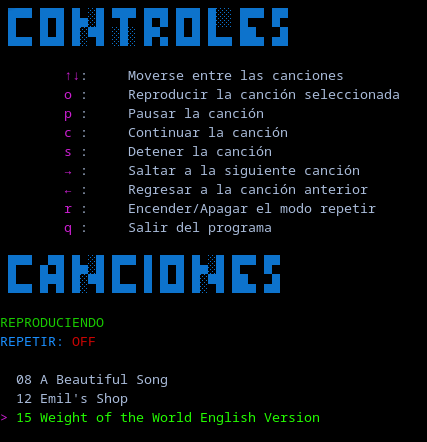
\includegraphics[width=8cm]{img/musica.png}
    \\
    \justifying
    \noindent
    Al ejecutar el comando \textit{musica} tendremos acceso a un reproductor de archivos mp3 dentro del cual podemos reproducir canciones en un directorio específico. Este reproductor utiliza como base el programa mpg123, por lo que al ejecutarlo lo primero que hará es verificar que esté instalado y, si no lo está, lo instalará.
    \\\\ 
    Si al ejecutar el programa no se le da un directorio como argumento, el programa lo solicitará con el siguiente mensaje:
    \\
    
    \centering
    
\includegraphics[width=16cm]{img/musica_prompt.png}
    \\
    \justifying
    \noindent
    Si no se encuentra ningún archivo mp3, el programa simplemente se cerrará.
    \\\\
    Dentro del menú. el usuario puede utilizar las diferentes teclas para navegar a través de su biblioteca, estas opciones son:
    \begin{itemize}
        \item Moverse entre canciones (flecha arriba/abajo)
        \item Reproducir la canción seleccionada
        \item Pausar la canción
        \item Continuar con la canción
        \item Saltar a la siguiente canción
        \item Regresar a la canción anterior
        \item Encender/Apagar el modo repetir
        \item Salir del programa
    \end{itemize}
    \\
    Dentro de la itnerfaz se puede ver el estado de reproducción (si está pausado o no), si está encendido el modo repetir y las canciones disponibles; si se está reproduciendo alguna canción se ilumina en verde.
    \textbf{Código:}
    \\
    \begin{lstlisting}[style=BashInputStyle]
#!/bin/bash

# Verify mpg123 installation, if not installed, try to install it
if ! which mpg123 >/dev/null; then
        echo -e "
        ->\e[31m ADVERTENCIA: NO TIENES INSTALADO EL PAQUETE mpg123
	\e[37mPara ejecutar esta función necesitas instarlo"
	read -p "	Deseas instalarlo?(y/n):" input
	if [ $input != "n" ] && [ $input != "N" ]
	then
	        echo -e "
		\e[37mDetectando distribución de Linux para instalar la dependencia..."
	        packagesNeeded='curl jq'
	        if [ -x "$(command -v apk)" ]
	                then sudo apk add --no-cache mpg123
	        elif [ -x "$(command -v apt-get)" ]
	                then sudo apt-get install mpg123
	        elif [ -x "$(command -v dnf)" ]
	                then sudo dnf install mpg123
	        elif [ -x "$(command -v zypper)" ]
	                then sudo zypper install mpg123
	        elif [ -x "$(command -v pacman)" ]
	                then sudo pacman -S mpg123
	        else
	                echo -e "
	->\e[31mERROR: No se pudo instalar el paquete mpg123
	\e[37mPara continuar, instala manualmente el programa
	        \e[0m"
	                exit
        	fi
	fi
fi

# Ask for playist path if not already given
if [ -z "$1" ] || [ "$1" -eq "" ] ; then 
	read -p $'
	\e[37mIngresa la ruta de dónde se encuentran las canciones\e[2m(presiona enter si es en el directorio actual)\e[0m: ' path
	if [ -z "$path" ] ; then # Assign current one if it's empty
		path=$(pwd)
	fi
else
	path=$1
fi
if [[ $path  != "/"* ]] ; then 
	path=$(pwd)/$path/
fi
if [ ! -d $path ] ; then
	echo -e "
        ->\e[31mERROR: No existe el directorio
        \e[37mCerrando programa...
        \e[0m"
        exit
fi

# Search for songs inside chosen path
i=0
songs=()
song_names=()
for file in $path*
do
    if [ "${file##*.}" == "mp3" ] ; then
	echo "Found song: $file"
	# Add song to the array
	songs+=("$file")
	song_name=("$(basename "$file")")
	song_names+=("${song_name::-4}")
	i+=1
    fi
done
if [ $i == 0  ] ; then # No songs detected causes the program to close
	echo -e "
    	->\e[31mERROR: No hay archivos .mp3 en el directorio
        \e[37mCerrando programa...
	\e[0m"
else

	# Menu cycle
	selected=0
	current_song=-1
	loop=false
	pausa=false
	pid=""
	echo "" > tmp # tmp file to store name of the current song


	# Play function
	function play(){
		# Play the selected song
		while true ; do
			echo "${song_names[$current_song]}" > tmp # Save the name of the current song
			mpg123 -q "${songs[$current_song]}" # Play the song	
			# Increase counter
			current_song=$((current_song+1))
			# If loop is not enabled break the cycle, if not go back to the first song
			if [ $current_song == $i ] ; then
				if [ $loop == false ] ; then
					echo "" > tmp # Clear tmp file
					break
				else
					current_song=0
				fi
			fi
		done
	}
	# Kill track
	function kill_track(){
		# Kill the current song
		if [ $current_song != -1 ] ; then
			kill $pid
		fi
		pkill mpg123
	}
	while true ; do
		# Clear the screen
		clear

		# Show controls
		echo -e " \e[34m█▀▀ █▀█ █▄░█ ▀█▀ █▀█ █▀█ █░░ █▀▀ █▀
	 █▄▄ █▄█ █░▀█ ░█░ █▀▄ █▄█ █▄▄ ██▄ ▄█
		\e[35m↑↓\e[0m: 	Moverse entre las canciones
		\e[35mo\e[0m : 	Reproducir la canción seleccionada
		\e[35mp\e[0m : 	Pausar la canción
		\e[35mc\e[0m : 	Continuar la canción
		\e[35ms\e[0m : 	Detener la canción
		\e[35m→\e[0m : 	Saltar a la siguiente canción
		\e[35m←\e[0m : 	Regresar a la canción anterior
		\e[35mr\e[0m : 	Encender/Apagar el modo repetir
		\e[35mq\e[0m : 	Salir del programa
		"

		# Show songs title
		echo -e " \e[34m█▀▀ ▄▀█ █▄░█ █▀▀ █ █▀█ █▄░█ █▀▀ █▀
	 █▄▄ █▀█ █░▀█ █▄▄ █ █▄█ █░▀█ ██▄ ▄█
	"

		# Show playing status
		if [ $current_song != -1 ] ; then
			if [ $pausa == true ] ; then
				echo -e "\e[31mPAUSADO"
			else
				echo -e "\e[32mREPRODUCIENDO"
			fi
		fi

		# Show current loop status
		if [ $loop == true ] ; then
			echo -e "\e[94mREPETIR: \e[32mON\e[0m
			"
		else
			echo -e "\e[94mREPETIR: \e[31mOFF\e[0m
			"
		fi
	
	    # Show available songs
		for i in "${!song_names[@]}"; do
			if [[ $i -eq $selected ]]; then
	        	# Highlight the selected file with a ">" symbol
		        printf "\e[35m> "
			else
				printf "  "
			fi
			# Compare current song with the one in the tmp file
			if [ "${song_names[$i]}" == "$(cat tmp)" ] ; then
		        	# Highlight the currently playing song in green
			        printf "\e[92m%s\n\e[0m" "${song_names[$i]}"
			else
	        		printf "\e[0m%s\n" "${song_names[$i]}"
		    fi
	    done
	
		# Read a single character from the user
	    read -rsn1 -d '' input
		# Execute actions based on the user input
		case $input in
			'q')  # Quit
				kill_track
				rm tmp
				clear
				break
				;;
			$'A')  # Up arrow
			        if [ $selected -gt 0 ] ; then
					selected=$((selected - 1))
				fi
				;;
			$'B')  # Down arrow
				if [[ $selected -lt $i ]] ; then
					selected=$((selected + 1))
				fi
				;;
			# Play selected song
			 $'o')
			 	# Change status
			 	pausa=false
	    		# Kill previous track
	    		kill_track
	    		# Play selected song
	    		current_song=$selected
				play & pid=$!
				;;
	        $'p') # Pause
				# Change status
			 	pausa=true
				kill -STOP $(pgrep mpg123) > /dev/null 2>&1
				;;
			$'c') # Continue
				# Change status
			 	pausa=false
				kill -CONT $(pgrep mpg123) > /dev/null 2>&1
				;;
			$'s') # Stop
				# Change status
			 	pausa=true
				# Kill previous track
				kill_track
				current_song=-1
				;;
			$'C') # Next
				# Change status
			 	pausa=false
				# Kill previous track
				kill_track
				# Find next song
				if [ $current_song -lt $i ] ; then
					current_song=$((current_song + 1))
					play & pid=$!
				elif [ $current_song -eq $i ] ; then
					if [ $loop == true ] ; then
						current_song=0
						play & pid=$!
					else
						current_song=-1
						pausa=true
						echo "" > tmp # Clear tmp file
					fi
				fi	
				;;
			$'D') # Back
				# Change status
			 	pausa=false
				# Kill previous track
				kill_track
				# Find previous song
				if [ $current_song -eq -1 ] ; then
					current_song=$i
				elif [ $current_song -eq 0 ] ; then
					if [ $loop == true ] ; then
						current_song=$i
					else
						current_song=0
					fi
				else
					current_song=$((current_song - 1))
				fi
				play & pid=$!
				;;
			$'r') # Repeat
				if [ $loop == false ] ; then
					loop=true
				else
					loop=false
				fi
				;;	
	    esac
	done
fi
reset
    \end{lstlisting}
    \textbf{Sintaxis:}
    \begin{lstlisting}[style=BashInputStyle]
musica
musica directorio_con_archivos_mp3
    \end{lstlisting}
    \textbf{Explicación del código: } \\
    Lo primero que realiza el programa es verificar que mpg123 esté instalado: sí no lo está intentará instalarlo utilizando algunos de los diferentes manejadores de paquetes, si no lo encuentrá se le dirá al usuario que no lo encontró y se le solicitará que lo haga para después cerrar el programa.
    \\\\
    Tras cumplir con el requerimiento de tener mpg123 instalado, se verificará si el usuario dió o no un directorio al llamar al programa, si no lo dió se le solicitará que lo haga. Si el directorio no existe, se cerrará el programa. Si se pudo abrir el directorio exitósamentes se recorrerán todos los archivos de este para ir almacenando los diferentes archivos mp3 que se encuentren; si no se encuentra ninguno el programa se cerrará.
    \\\\
    Se inicializarán entonces algunas variables que nos ayudarán a llevar la cuenta de qué canción está seleccionada por el cursor,  la canción en reproducción, si la canción está pausada, si está encendido el modo de repetició y el pid del proceso que ejecutará las canciones, adicionalmente, se creará un archivo llamado \textit{tmp} donde se almacenará la canción en reproducción; la razón por la que tuvimos que usar un archivo es porque la reproducción y el menú utilizan dos procesos distintos y la mejor forma que encontramos para que se comunicaran entre sí es mediante un archivo.
    \\\\
    Entraremos entonces en un ciclo eterno donde primero se le muestran las opciones disponibles al usuario y luego la lista de canciones (incluyendo el cursor y la que se está reproduciendo), los estados del reproductor (si está en pausa y/o  en repetición) para después esperar a que presione alguna tecla. Al presionar una tecla, puede realizarse lo siguiente dependiendo de cual sea:
    \begin{itemize}
        \item \textbf{q} \\
        Se detiene la reproducción de canciones, se borra el archivo temporal y se rompe el ciclo.
        \item \textbf{Tecla arriba} \\
        Se mueve el cursor hacia arriba.
        \item \textbf{Tecla abajo} \\
        Se mueve el cursor hacia abajo.
        \item \textbf{o} \\
        Se detiene la reproducción anterior, se cambia el estado de pausa a falso y se reproduce la canción actual en un proceso paralelo; el pid del proceso paralelo se almacena para que sea posible detener la reproducción en cuanto otra quiera tomar su lugar.
        \item \textbf{p} \\
        Pausa la reproducción y cambia el estado de pausa a verdadero.
        \item \textbf{c} \\
        Reanuda la reproducción y cambia el estado de pausa a falso.
        \item \textbf{s} \\
        Cancela la reproducción y cambia el estado de pausa a verdadero.
        \item \textbf{Tecla derecha} \\
        Se detiene la reproducción anterior, se cambia el estado de pausa a falso y se reproduce la canción siguiente a la que estaba; el pid del proceso paralelo se almacena para que sea posible detener la reproducción en cuanto otra quiera tomar su lugar. Si se trata de la última canción se repetirá el ciclo si el modo de repetición está activado, de lo contrario, la reproducción se detendrá.
        \item \textbf{Tecla izquierda} \\
        Se detiene la reproducción anterior, se cambia el estado de pausa a falso y se reproduce la canción anterior a la que estaba; el pid del proceso paralelo se almacena para que sea posible detener la reproducción en cuanto otra quiera tomar su lugar. Si se trata de la última canción se reproducirá la última canción si si el modo de repetición está activado, de lo contrario, se repetirá la primera canción.
        \item \textbf{r} \\
        Activa o desactiva el modo de repetición.
    \end{itemize}
    
    \newpage
\section{Conclusiones}
\justifying
\noindent
\begin{itemize}
    \item \textbf{Rodríguez García Javier Antonio} \\
    A lo largo de la realización del programa, se me precentaron muchos percances, uno de ellos fue el inicio de sesion, pues la contraseña se encuentra cifrada, para evitar estos problemas, tuve que buscar muchas alternativas, sin embargo, al final consegui los objetivos, en lo personal, el proyecto me ayudo mucho a mejorar mis capacidades de investigación y de programación en bash, ademas de contribuir en la mejora de mi logica al programar, una de las cosas que mas me gustaron fue la implementación del ascii art, pues me parece que darle un toque colorido al codigo hacer que se vea mejor y mas elaborado, otra cosa que me llamo la atencion, fue que en bash se peuden mandar llamar funciones con argumentos sin neceisdad de declararlos, lo que facilito muchas implementaciones.   
    \item \textbf{Treviño Selles Jorge Eithan} \\
    Durante este proyecto aprendí bastante y me familiaricé más con el lenguaje de programación Bash y los diferentes componentes del sistema operativo GNU/Linux. Realmente fue un proyecto que requirió de mucha investigación, tiempo y percepción cuando surgían errores. Afortunadamente el proyecto fue elaborado en equipos por lo que la carga de trabajo no fue tan alta, sin embargo, el trabajar en equipo también implica un balance y una comunicación clara de quién va a desarrollar qué parte y las diferentes convenciones a seguir. En general, puedo decir que fue un proyecto bastante didáctico e incluso desafiante en algunos puntos como lo fue el reproductor de música ya que ponía a prueba mis conocimientos de diferentes temas (sistemas operativos, estructuras de datos, etc).
\end{itemize}

\end{document}